\documentclass[paper=a4, fontsize=11pt]{scrartcl}

\usepackage{hyperref}
\usepackage{listings}
\usepackage{cite}
\usepackage{booktabs} % Required for better horizontal rules in tables
\usepackage{multirow}
\usepackage{multicol}
\usepackage{graphicx}
\usepackage{enumitem}
\usepackage{lscape}

\lstset{
	sensitive=false,    % not case-sensitive
	morecomment=[l]{;;}, % line comment
	alsoletter={:,-},   % consider extra characters
	frame=single,
	%numbers=left,
	breaklines=true,
	tabsize=2,
	basicstyle=\footnotesize,
}

\setlength\parindent{0pt}

\title{MAAS Project: Flying Saucers Bakery}
\author{ \'{A}ngela Patricia Enr\'{i}quez G\'{o}mez \\
	Erick Romero Kramer \\
	Ethan Massey }

\begin{document}
	
	\maketitle
	
	\section{Introduction}
	
	In this project, the production of a bakery is simulated using JADE, a software framework for developing multi-agent systems \cite{Bellifemine}. \\
	
	The workflow of the bakery is divided into 5 preparation stages: 
	
	\begin{itemize}
		\item Order processing
		\item Dough preparation
		\item Baking
		\item Packaging
		\item Delivery
	\end{itemize}
	
	All agents extend a BaseAgent class, which provides the system clock. A production action is allowed every time step. \\
	
	We have developed and implemented two production stages: Dough preparation and Baking. The interface agent of the Packaging stage has been integrated at the end of our Baking stage to allow testing of the remaining stages. A DummyOrderProcessor is the entry agent of our system. We call it dummy because it does not schedule orders based on the production of each bakery, nor does it compare the prices of the bakeries before placing an order. The DummyOrderProcessor reads the orders (contained in the file clients.json), randomly selects a bakery ID and sends the order to the DoughManager and the BakingInterface of the selected bakery ID. \\
	
	
\begin{landscape}
	
	\begin{figure}
	\centering
	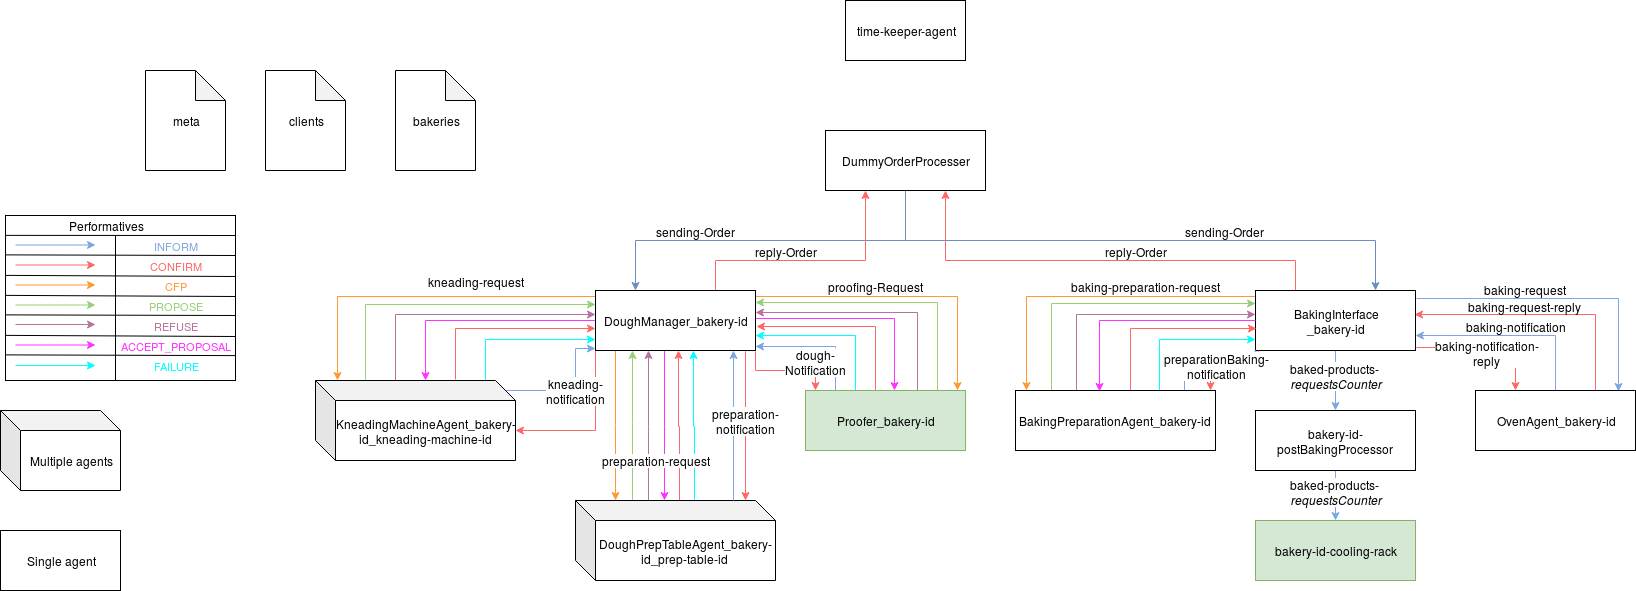
\includegraphics[width=1\linewidth]{images/architecture}
	\caption{Architecture of the Bakery JADE multi-agent system.}
	\label{fig:architecture}
	\end{figure}

\end{landscape}

		\section{System architecture}
		
		Table \ref{fig:architecture} shows the architecture of the Bakery JADE multi-agent system. Each rectangle represents an agent and the 
		interface agents are colored in green. The files bakeries.json contains the bakery information, while the meta.json has the the time step information. The orders are stored in the clients.json files. 



	\section{Agents}
	
		Table \ref{table-agents} shows the agents in system, the number of instances of each agent and the method used for creating them. The DummyOrderProcesser, DoughManager agents, Proofer, BakingInterface agents and CoolingRackAgent are created by the Start.java file. Each production stage uses an argument in the Start.java which calls the Initializer of that particular stage. The DougManager creates the agents used in the dough preparation stage, expect for the proofer. Similarly, the BakingInterface creates the agents of the bakery stage, except for the CoolingRackAgent. 
		
	
	\begin{table}[h!]	
		\centering
		\small
		
		\begin{tabular}{llll}
			\toprule   
			
			Production Stage & Agent  & Created by & Number of instances \\
			\midrule
			
			\multirow{1}{*} {Order Processing} &
			
			{DummyOrderProcesser} &
			
			DoughPrepStageInitializer & 1 \\
			
			
			\cmidrule(l){1-4}
			
			\multirow{7}{*} {Dough Preparation} &
			
			{DoughManager} &
			
			 DoughPrepStageInitializer & 1 per bakery ID \\
			 
			 \cmidrule(l){2-4} 
			 
			 {} & KneadingMachineAgent & DoughManager & {\shortstack[l]{$n$ per bakery ID, where $n$ \\ is taken from bakeries.json}} \\
			 
			  \cmidrule(l){2-4} 
			  
			  {} & DoughPrepTableAgent & DoughManger & {\shortstack[l]{$n$ per bakery ID, where $n$ \\ is taken from bakeries.json}} \\
			  
			  \cmidrule(l){2-4} 
			  
			  {} & Proofer & DoughPrepStageInitializer &  1 per bakery ID \\
			  
			 \midrule
			  
			 \multirow{7}{*} {Baking} &
			 
			 {BakingInterface} &
			 
			 BakingMasMaasInitializer & 1 per bakery ID \\
			 
			 \cmidrule(l){2-4} 
			 
			 {} & OvenAgent & BakingInterface & 1 per bakery ID \\
			 
			 \cmidrule(l){2-4} 
			 
			 {} & BakingPreparationAgent & BakingInterface & 1 per bakery ID \\
			 
			 \cmidrule(l){2-4} 
			 
			 {} & PostBakingProcessor & BakingInterface &  1 per bakery ID \\
			 
			 \cmidrule(l){2-4} 
			 
			 {} & CoolingRackAgent & BakingStageInitializer &  1 per bakery ID \\
			
			\bottomrule
		\end{tabular}
		\caption{Agents in the Bakery JADE.} 
		\label{table-agents}
	\end{table}
	
	\subsection{Description of the Agents}
	
	\begin{itemize}
		\item \textbf{DummyOrderProcesser.} Reads the orders, randomly selects a bakery ID and sends the order to the DoughManager and BakingInterface agents of the selected bakery ID. \\
		
		\item \textbf{DoughManager.} Creates the KneadingMachine and DoughPrepTable agents according to the information on the bakery.json. Aggregates orders by product type and maintains queues of products that need kneading, need preparation and need proofing. Coordinates the whole dough preparation stage.  \\
		
		\item \textbf{KneadingMachineAgent.} Receives CFPs for performing kneading. If the agent is available, it sends a PROPOSE. If the agent is already kneading, it sends a REFUSE. 
		
		The KneadingMachine starts kneading when it receives an ACCEPT\_PROPOSAL. The agent can only accept a new \textit{Kneading Request} once it has finished its previous request. When the KneadingMachine agent is done, it sends a \textit{Kneading Notification} to the DoughManager. \\
		
		\item \textbf{DoughPrepTableAgent} Receives CFPs for performing dough preparation. If the agent is available, it sends a PROPOSE. If the agent is already preparing products, it sends a REFUSE. 
		
		The DoughPrepTableAgent starts executing the preparation steps when it receives an ACCEPT\_PROPOSAL. The agent can only accept a new \textit{Preparation Request} once it has finished its previous request. When the DoughPrepTableAgent agent is done, it sends a \textit{Preparation Notification} to the DoughManager. 
		
		\item \textbf{Proofer.} Receives CFPs for proofing. If the agent is available, it sends a PROPOSE. If the agent is already proofing, it sends a REFUSE. 
		
		The Proofer starts proofing when it receives an ACCEPT\_PROPOSAL. The agent can only accept a new \textit{Proofing Request} once it has finished its previous request. When the Proofer agent is done, it sends a \textit{Dough Notification} to the BakingInterface agent. The Proofer is the interface agent between the dough and the baking stages. \\
		
		\item \textbf{BakingInterface.} Creates the Oven, the BakingPreparation and the PostBakingProcessor agents. Aggregates orders per product type and maintains queues of products that neeed baking and need preparation. Coordinates the whole baking stage and sends \textit{Cooling Request} messages to the PostBakingProcessor agent of the bakery ID. \\
		
		\item \textbf{OvenAgent.} Receives \textit{Baking Request} messages, and replies sending a CONFIRM. It books slots for each baking request. Once a slot has reached the desired temperature, the products are baked. After the baking time is over, the OvenAgent creates and sends a \textit{Baking Notification} containing information of the products that were baked. \\
		
		\item \textbf{BakingPreparationAgent.} Receives CFPs for performing baking preparation. If the agent is available, it sends a PROPOSE. If the agent is already preparing products, it sends a REFUSE. 
		
		The BakingPreparationAgent starts executing the preparation steps when it receives an ACCEPT\_PROPOSAL. The agent can only accept a new \textit{Baking Preparation Request} once it has finished its previous request. When the BakingPreparationAgent is done, it sends a \textit{Baking Preparation Notification} to the DoughManager. \\ 
			
		\item \textbf{PostBakingProcessor.} Receives a \textit{Cooling Request} message from the BakingInterface and resends it to the CoolingRackAgent. The message sent to the CoolingRackAgent is called \textit{Loading Bay} message but it contains the same information as the \textit{Cooling Request} message. \\
		
		\item \textbf{CoolingRackAgent.} Receives \textit{Loading Bay} messages from the PostBakingProcessor agent and performs cooling. It is the interface agent of the next stage.
		
	\end{itemize}
	\newpage
	\section{Objects}
	demo
	\begin{table}[http!]	
		\centering
		\small
		
		\begin{tabular}{llll}
			\toprule   
			
			Object  & Parent class & Members type & Members \\
			\midrule
			
					
			\multirow{4}{*} {OrderMas} & & String & customer\_id \\
							&		 &	 String & guid \\
						     &       &   OrderDate & order\_date \\
							&		 &   DeliveryDate & delivery\_date\\
						     &      &   Vector$<$BakedGood$>$ & products \\
			\midrule
			\multirow{2}{*} {OrderDate} & & int & day \\
							&		 &	 int & hour \\
			\midrule
			\multirow{2}{*} {DeliveryDate} & & int & day \\
									 & &	 int & hour \\		
						
			\midrule	
			\multirow{3}{*} {BakedGood} & & String & name \\
			&	& int & amount \\
			&   &String [ ] & bakedGoodNames \\
			
			\midrule
			\multirow{6}{*} {Bakery} & &String & guid \\
			&	 &String & name \\
			&   &Point2D & location \\
			& &Vector$<$ProductMas$>$ & products \\
			& &Vector$<$String$>$ & availableProducts \\
			& &Vector$<$Equipment$>$ & equipment \\
			
			\midrule
			\multirow{6}{*} {ProductMas} & &String & guid \\
			&	 & Batch & batch \\
			&   & Recipe & recipe \\
			& & Packaging & packaging \\
			& &Double & salesPrice \\
			& & Double & productionCost \\
			
			\midrule
			\multirow{6}{*} {Bakery} & &String & guid \\
			&	 & String & name \\
			&   & Point2D & location \\
			& & Vector$<$ProductMas$>$ & products \\
			& & Vector$<$String$>$ & availableProducts \\
			& & Vector$<$Equipment$>$ & equipment \\
			
			\midrule
			\multirow{2}{*} {Equipment} & & String & guid \\
			&	 & boolean & isAvailable \\
			
			\midrule
			\multirow{1}{*} {Batch} &  & int & breadsPerOven \\
			
			\midrule
			\multirow{3}{*} {CoolingRequestTuple} & & String & guid \\
			&	& int & quantity \\
			&   & float & coolingDuration \\
			
			\midrule
			\multirow{1}{*} {DoughPrepTable} & Equipment & &  \\
			
			\midrule
			\multirow{1}{*} {KneadingMachine} & Equipment & &  \\
			
			\midrule
			\multirow{4}{*} {Oven} & Equipment & int & NUM\_SLOTS  \\
			& & int & coolingRate \\
			& & int & heatingRate \\
			& & Vector$<$OvenSlot$>$ & ovenSlots \\
					
			\bottomrule
		\end{tabular}
		\caption{Objects in the Bakery JADE. Part 1.} 
		\label{table-objects1}
	\end{table}
	
	\newpage
	\begin{table}[http!]	
		\centering
		\small
		
		\begin{tabular}{llll}
			\toprule   
			
			Object  & Parent class & Members type & Members \\
			\midrule
			
			
			\multirow{13}{*} {OvenSlot} & & float & STARTING\_TEMP \\
			&		 &	 float & currentTemp \\
			&       &   String & ovenGuid \\
			&		 &   String & guid\\
			&      &   Integer & quantity \\
			& 	   &   boolean & available \\
			& & boolean & readyToBake \\
			& & String & productType \\
			& & int & coolingRate \\
			& & int & heatingRate \\
			& & float & bakingTime \\
			& & float & bakingTemp \\
			& & int & bakingCounter \\
			
			\midrule
			\multirow{4}{*}{ProductStatus} & & String & guid \\
			& & String & Status\\
			& & int & amount \\
			& & productMas & product \\			

			\midrule
			\multirow{2}{*}{Recipe} & & int & bakingTemp \\
			& & Vector<Steps> & steps\\
			
			\midrule
			\multirow{7}{*}{Step} & & String & action \\
			& & Float & duration\\
			& & String & KNEADING\_STEP \\
			& & String & ITEM\_PREPARATION\_STEP \\
			& & String & PROOFING\_STEP \\
			& & String & BAKING\_STEP \\
			& & String & COOLING\_STEP \\
			
			\midrule 
			\multirow{1}{*}{WorkQueue} & & LinkedList$<$ProductStatus$>$ & workQueue \\
			\bottomrule
		\end{tabular}
		\caption{Objects in the Bakery JADE. Part 2.} 
		\label{table-objects2}
	\end{table}
	
	\section{Behaviours}
	
	Tables \ref{table-behaviours1} and \ref{table-behaviours2} show the behaviors that each agent activates.
	
	\begin{table}[h!]	
		\centering
		\small
		
		\begin{tabular}{llll}
			\toprule   
			
			Production Stage & Agent  & Behaviour Name & Behaviour Type \\
			\midrule
			
			\multirow{2}{*} {Order Processing} &
			
			\multirow{2}{*} {DummyOrderProcesser} &
			
			timeTracker & CyclicBehaviour \\
			
			\cmidrule(l){3-4}
			
			{} & {} & sendOrder & Behaviour \\
			
			\cmidrule(l){1-4}
			
			\multirow{35}{*} {Dough Preparation} &
			
			\multirow{15}{*} {Dough Manager} &
			
			timeTracker & CyclicBehaviour \\
			
			\cmidrule(l){3-4}
			
			{} & {} & ReceiveOrders & CyclicBehaviour \\
			
			\cmidrule(l){3-4}
			
			{} & {} & checkingKneadingWorkqueue & CyclicBehaviour \\
			
			\cmidrule(l){3-4}
			
			{} & {} & checkingPreparationWorkqueue & CyclicBehaviour \\
			
			\cmidrule(l){3-4}
			
			{} & {} & checkingProofingWorkqueue & CyclicBehaviour \\
			
			\cmidrule(l){3-4}
			
			{} & {} & RequestKneading & Behaviour \\
			
			\cmidrule(l){3-4}
			
			{} & {} & RequestPreparation & Behaviour \\
			
			\cmidrule(l){3-4}
			
			{} & {} & RequestProofing & Behaviour \\
			
			\cmidrule(l){3-4}
			
			{} & {} & ReceiveKneadingNotification & CyclicBehaviour \\
			
			\cmidrule(l){3-4}
			
			{} & {} & ReceivePreparationNotification & CyclicBehaviour \\
			
			\cmidrule(l){2-4}
			
			{} & \multirow{7}{*} {KneadingMachineAgent} &
			
			timeTracker & CyclicBehaviour \\
			
			\cmidrule(l){3-4}
			
			{} & {} & ReceiveProposalRequests & CyclicBehaviour \\
			
			\cmidrule(l){3-4}
			
			{} & {} & ReceiveKneadingRequests & CyclicBehaviour \\
			
			\cmidrule(l){3-4}
			
			{} & {} & Kneading & OneShotBehaviour \\
			
			\cmidrule(l){3-4}
			
			{} & {} & SendKneadingNotification & Behaviour \\
			
			\cmidrule(l){2-4}
			
			{} & \multirow{7}{*} {DoughPrepTableAgent} &
			
			timeTracker & CyclicBehaviour \\
			
			\cmidrule(l){3-4}
			
			{} & {} & ReceiveProposalRequests & CyclicBehaviour \\
			
			\cmidrule(l){3-4}
			
			{} & {} & ReceivePreparationRequests & CyclicBehaviour \\
			
			\cmidrule(l){3-4}
			
			{} & {} & Preparation & OneShotBehaviour \\
			
			\cmidrule(l){3-4}
			
			{} & {} & SendPreparationNotification & Behaviour \\
			
			\cmidrule(l){2-4}
			
			{} & \multirow{7}{*} {Proofer} &
			
			timeTracker & CyclicBehaviour \\
			
			\cmidrule(l){3-4}
			
			{} & {} & ReceiveProposalRequests & CyclicBehaviour \\
			
			\cmidrule(l){3-4}
			
			{} & {} & ReceiveProofingRequests & CyclicBehaviour \\
			
			\cmidrule(l){3-4}
			
			{} & {} & Proofing & OneShotBehaviour \\
			
			{} & {} & SendDoughNotification & Behaviour \\
			
			\bottomrule
		\end{tabular}
		\caption{Behaviours in the Bakery JADE. Part 1.} 
		\label{table-behaviours1}
	\end{table}
	
	\begin{table}[h!]	
		\centering
		\small
		
		\begin{tabular}{llll}
			\toprule   
			
			Production Stage & Agent  & Behaviour Name & Behaviour Type \\
			\midrule
			
			\multirow{33}{*} {Baking} &
			
			\multirow{13}{*} {BakingInterface} &
			
			timeTracker & CyclicBehaviour \\
			
			\cmidrule(l){3-4}
			
			{} & {} & ReceiveOrders & CyclicBehaviour \\
			
			\cmidrule(l){3-4}
			
			{} & {} & ReceiveDoughNotification & CyclicBehaviour \\
			
			\cmidrule(l){3-4}
			
			{} & {} & checkingBakingWorkqueue & CyclicBehaviour \\
			
			\cmidrule(l){3-4}
			
			{} & {} & checkingPreparationWorkqueue & CyclicBehaviour \\
			
			\cmidrule(l){3-4}
			
			{} & {} & RequestBaking & Behaviour \\
			
			\cmidrule(l){3-4}
			
			{} & {} & RequestPreparation & Behaviour \\
			
			\cmidrule(l){3-4}
			
			{} & {} & RequestCooling & Behaviour \\
			
			\cmidrule(l){3-4}
			
			{} & {} & ReceiveBakingNotification & CyclicBehaviour \\
			
			\cmidrule(l){3-4}
			
			{} & {} & ReceivePreparationNotification & CyclicBehaviour \\
			
			\cmidrule(l){2-4}
			
			{} & \multirow{7}{*} {OvenAgent} &
			
			timeTracker & CyclicBehaviour \\
			
			\cmidrule(l){3-4}
			
			{} & {} & ReceiveBakingRequests & CyclicBehaviour \\
			
			\cmidrule(l){3-4}
			
			{} & {} & checkingBakingRequests & CyclicBehaviour \\
			
			\cmidrule(l){3-4}
			
			{} & {} & Baking & OneShotBehaviour \\
			
			\cmidrule(l){3-4}
			
			{} & {} & SendBakingNotification & Behaviour \\
			
			\cmidrule(l){2-4}
			
			{} & \multirow{7}{*} {BakingPreparationAgent} &
			
			timeTracker & CyclicBehaviour \\
			
			\cmidrule(l){3-4}
			
			{} & {} & ReceiveProposalRequests & CyclicBehaviour \\
			
			\cmidrule(l){3-4}
			
			{} & {} & ReceivePreparationRequests & CyclicBehaviour \\
			
			\cmidrule(l){3-4}
			
			{} & {} & Preparation & OneShotBehaviour \\
			
			\cmidrule(l){3-4}
			
			{} & {} & SendPreparationNotification & Behaviour \\
			
			\cmidrule(l){2-4}
			
			{} & \multirow{3}{*} {PostBakingProcessor} &
			
			timeTracker & CyclicBehaviour \\
			
			\cmidrule(l){3-4}
			
			{} & {} & ReceiveAndRequestCooling & CyclicBehaviour \\

			\bottomrule
		\end{tabular}
		\caption{Behaviours in the Bakery JADE. Part 2.} 
		\label{table-behaviours2}
	\end{table}
	
	\subsection*{Shared Behaviours}
	
	\begin{itemize}
		\item \textbf{timeTracker.} All the agents share this behaviour, which checks if the agents are allowed to perform an action. Once the agents are done with an action, they inform the TimeKeeper agent by calling the finished method of the baseAgent. Agents are done with the action of a time step only if they are not currently processing a message. Moreover, the timeTracker behaviour checks if the bakery is in production hours. The production time is from midnight to lunch (00.00 hours to 12 hours). 
		
	\end{itemize}
	
	\subsection*{DummyOrderProcesser Behaviours}
	
	\begin{itemize}
		
		\item \textbf{sendOrder.} Sends an \textit{Order} message to the DoughManager and BakingInterface agents of a bakery ID. The order message is sent using the INFORM performative. The behaviour expects an ACL.CONFIRM message from both agents. 
		
	\end{itemize}
	
	\subsection*{DoughManager Behaviours}
	
	\begin{itemize}
		
		\item \textbf{ReceiveOrders.} Receives a ACL.INFORM \textit{Order} message from the DummyOrderProcesser and replies with a ACL.CONFIRM message. It adds the orders to a queue of orders.
		
		\item \textbf{checkingKneadingWorkqueue.} Aggregates the orders that need kneading by product type and creates a \textit{Kneading Request} message. Converts the \textit{Kneading Request} to Json string and activates a RequestKneading behaviour for the \textit{Kneading Request}. 
		
		\item \textbf{checkingPreparationWorkqueue.} Aggregates the orders that need preparation by product type and creates a \textit{Preparation Request} message. Converts the \textit{Preparation Request} to Json string and activates a RequestPreparation behaviour for the \textit{Preparation Request}.
		
		\item \textbf{checkingProofingWorkqueue.} Aggregates the orders that need proofing by product type and creates a \textit{Proofing Request} message. Converts the \textit{Proofing Request} to Json string and activates a RequestProofing behaviour for the \textit{Proofing Request}.
		
		\item \textbf{RequestKneading.} Sends a CFP for a \textit{Kneading Request} to all the KneadingMachine agents. Sends an ACCEPT\_PROPOSAL to the first KneadingMachine agent that replied to the CFP with a PROPOSE message and expects an INFORM message as reply. If the CFP fails, i.e., if no KneadingMachine sent a proposal or if the assigned KneadingMachine did no reply with an inform, the products used to create the \textit{Kneading Request} are added back to the needsKneading workqueue. 
		
		\item \textbf{RequestPreparation.} Sends a CFP for a \textit{Preparation Request} to all the DoughPrepTable agents. Sends an ACCEPT\_PROPOSAL to the first DoughPrepTable agent that replied to the CFP with a PROPOSE message and expects an INFORM message as reply. If the CFP fails, i.e., if no DoughPrepTable sent a proposal or if the assigned DoughPrepTable did no reply with an inform, the products used to create the \textit{Preparation Request} are added back to the needsPreparation workqueue.
		
		\item \textbf{RequestProofing.} Sends a CFP for a \textit{Proofing Request} to the Proofer agent. If the Proofer agent replied to the CFP with a PROPOSE message, the DoughManager 
		sends an ACCEPT\_PROPOSAL and expects an INFORM message as reply. If the CFP fails, i.e., if the Proofer did not send a proposal or if it did no reply with an inform, the products used to create the \textit{Proofing Request} are added back to the needsProofing workqueue.
		
		\item \textbf{ReceiveKneadingNotification.} Receives an INFORM \textit{Kneading Notification} message and replies with a CONFIRM. Converts the \textit{Kneading Notification} Json string to an object and adds the kneaded products to the queue needsPreparation. 
		
		\item \textbf{ReceivePreparationNotification.} Receives an INFORM \textit{Preparation Notification} message and replies with a CONFIRM. Converts the \textit{Preparation Notification} Json string to an object and adds the prepared products to the queue needsProofing.
			
	\end{itemize}
	
	\subsection*{KneadingMachine Behaviours}
	
	\begin{itemize}
		\item \textbf{ReceiveProposalRequests.} Receives CFPs for performing kneading. If the KneadingMachine agent is already taken, it replies with a REFUSE and if it is free it sends a PROPOSE.
		
		\item \textbf{ReceiveKneadingRequests.} Receives ACCEPT\_PROPOSALs.  If the KneadingMachine agent has already accepted another request it replies with a FAILURE. If it is still available it replies with an INFORM, converts the \textit{Kneading Request} message to an object, extracts the information needed for kneading and activates the Kneading behaviour. 
		
		\item \textbf{Kneading.} Performs a kneading action if the kneading counter is less than the kneading time of the product being produced. This is a OnceShotBehaviour which is activated at every time step. Once the kneading counter is equal to the kneading time, the KneadingMachine stops kneading, becomes available and activates the SendKneadingNotification behaviour.  
		
		\item \textbf{SendKneadingNotification.} Sends an INFORM message with a \textit{Kneading Notification} to the DoughManager and expects a CONFIRM message as reply. 
	\end{itemize}
	
		\subsection*{PreparationTable Behaviours}
		
		\begin{itemize}
			\item \textbf{ReceiveProposalRequests.} Receives CFPs for performing preparation. If the DoughPrepTable agent is already taken, it replies with a REFUSE and if it is free it sends a PROPOSE.
			
			\item \textbf{ReceivePreparationRequests.} Receives ACCEPT\_PROPOSALs.  If the DoughPrepTable agent has already accepted another request it replies with a FAILURE. If it is still available it replies with an INFORM, converts the \textit{Preparation Request} message to an object, extracts the information needed for performing preparation and activates the Preparation behaviour. 
			
			\item \textbf{Preparation.} The preparation consists of several steps. This OnceShotBehaviour is activated at every time step and performs the preparation actions of each preparation step in a sequential manner. That is, it performs the preparation actions of the first step, then the preparation actions of the second step and so on until reaching the last step. It gets the duration of each preparation step and performs a preparation action each time step. Once the last preparation step has been completed, the PreparationTable stops preparing, becomes available and activates the SendPreparationNotification behaviour.  
			
			\item \textbf{SendPreparationNotification.} Sends an INFORM message with a \textit{preparation-notification} to the DoughManager and expects a CONFIRM message as reply. 
		\end{itemize}
		
		\subsection*{Proofer Behaviours}
		
		\begin{itemize}
			\item \textbf{ReceiveProposalRequests.} Receives CFPs for performing proofing. If the Proofer agent is already taken, it replies with a REFUSE and if it is free it sends a PROPOSE.
			
			\item \textbf{ReceiveProofingRequests.} Receives ACCEPT\_PROPOSALs.  If the Proofer agent has already accepted another request it replies with a FAILURE. If it is still available it replies with an INFORM, converts the \textit{Proofing Request} message to an object, extracts the information needed for proofing and activates the Proofing behaviour. 
			
			\item \textbf{Proofing.} Performs a proofing action if the proofing counter is less than the proofing time of the product being produced. This is a OnceShotBehaviour which is activated at every time step. Once the proofing counter is equal to the proofing time, the Proofer stops proofing, becomes available and activates the SendDoughNotification behaviour.  
			
			\item \textbf{SendDoughNotification.} Sends an INFORM message with a \textit{Dough Notification} to the BakingInterface agent and expects a CONFIRM message as reply. 
		\end{itemize}
		
	\subsection*{BakingManager Behaviours}
	
	\begin{itemize}
		\item  \textbf{ReceiveOrders.} Receives a ACL.INFORM \textit{Order} message from the DummyOrderProcesser and replies with a ACL.CONFIRM message. 
		
		\item  \textbf{ReceiveDoughNotification.} Receives \textit{Dough Notification} messages from the Proofer interface agent and stores the product type, guids and product quantities in a needs baking workqueue. 
		
		\item \textbf{checkingBakingWorkqueue.} Aggregates the orders that need baking by product type and creates a \textit{Baking Request} message. Converts the \textit{Baking Request} to Json string and activates the RequestBaking behaviour for the \textit{Baking Request}.
		
		\item \textbf{checkingPreparationWorkqueue.} Aggregates the orders that need preparation by product type and creates a \textit{Baking Preparation Request} message. Converts the \textit{Preparation Request} to Json string and activates a RequestPreparation behaviour for the \textit{Preparation Request}.
		
		\item \textbf{RequestBaking.} Sends an INFORM message containing a \textit{Baking Request} and receives a CONFIRM as reply.
		
		\item \textbf{RequestPreparation.} Sends a CFP for a \textit{Baking Preparation Request} to all the BakingPreparation agents. Sends an ACCEPT\_PROPOSAL to the first BakingPreparation agent that replied to the CFP with a PROPOSE message and expects an INFORM message as reply. If the CFP fails, i.e., if no BakingPreparation sent a proposal or if the assigned BakingPreparation did no reply with an inform, the products used to create the \textit{Baking Preparation Request} are added back to the needsPreparation workqueue.
		
		\item \textbf{RequestCooling.} Sends \textit{Cooling Request} messages to the PostBakingProcessor agent using an INFORM. Acts as a proxy between the BakingInterface and the CoolingRack agent. 
		
		\item \textbf{ReceiveBakingNotification.} Receives an INFORM \textit{Baking Notification} message and replies with a CONFIRM. Converts the \textit{Baking Notification} Json string to an object and adds the baked products to the queue needsPreparation. 
		
		\item \textbf{ReceivePreparationNotification.} Receives an INFORM \textit{Baking Preparation Notification} message and replies with a CONFIRM. Converts the \textit{Baking Preparation Notification} Json string to an object and creates \textit{Cooling Request} messages for the products that are done with the preparation stage. It activates a RequestCooling behaviour per \textit{Cooling Request}.
			
	\end{itemize}
	
	\subsection*{OvenAgent Behaviours}
	
	\begin{itemize}
		\item \textbf{ReceiveBakingRequest.} Receives and INFORM \textit{Baking Request} message and replies with a CONFIRM. Adds the received \textit{Baking Request} to a list of baking requests.
		
		\item \textbf{checkingBakingRequests.} Gets the first element in the list of baking requests and books the slots needed for baking the products of each order guid. If not all products of a guid could be assigned to a slot, the baking request is modified with the remaining products and added back to the list of baking requests.
		
		\item \textbf{Baking.} It heats, cools down the booked slots and bakes. If the slots have the baking temperature it bakes the products for the baking time specified in the recipes. This is a OnceShotBehaviour which is activated at every time step. Once the baking counter is equal to the baking time, the Oven stops baking, releases the slot and  and activates the SendBakingNotification behaviour.  
		
		\item \textbf{SendBakingNotification.} Sends a \textit{Baking Notification} of the products that have been baked and expects a CONFIRM.	
		
	\end{itemize}
	
		\subsection*{BakingPreparationAgent Behaviours}
		
		\begin{itemize}
			\item \textbf{ReceiveProposalRequests.} Receives CFPs for performing preparation. If the BakingPreparationAgent agent is already taken, it replies with a REFUSE and if it is free it sends a PROPOSE.
			
			\item \textbf{ReceivePreparationRequests.} Receives ACCEPT\_PROPOSALs.  If the BakingPreparationAgent agent has already accepted another request it replies with a FAILURE. If it is still available it replies with an INFORM, converts the \textit{Baking Preparation Request} message to an object, extracts the information needed for performing preparation and activates the Preparation behaviour. 
			
			\item \textbf{Preparation.} The preparation consists of several steps. This OnceShotBehaviour is activated at every time step and performs the preparation actions of each preparation step in a sequential manner. That is, it performs the preparation actions of the first step, then the preparation actions of the second step and so on until reaching the last step. It gets the duration of each preparation step and performs a preparation action each time step. Once the last preparation step has been completed, the BakingPreparationAgent stops preparing, becomes available and activates the SendPreparationNotification behaviour.  
			
			\item \textbf{SendPreparationNotification.} Sends an INFORM message with a \textit{Baking Preparation Notification} to the BakingInterface and expects a CONFIRM message as reply. 
		\end{itemize}
		
		\subsection*{BakingPreparationAgent Behaviours}
		
		\begin{itemize}
			\item \textbf{ReceiveAndRequestCooling.} Receives a \textit{Cooling Request} message from the BakingInterface and sends it to the Cooling Rack agent. 
		\end{itemize}
	

	\section{Messages}
	
	Table \ref{table-messages} shows the messages that the Bakery JADE sends for the order processing, dough and baking stages. Information about the performative, sender, receive and conversation ID is included in the table. All messages are sent as Json strings. In this section we present an example of each type of message. 
	
	\subsection{Order Processing Stage}
	
	 \textbf{Order}
\begin{lstlisting}
{
	"customer_id":"customer-001",
	"guid":"order-001",
	"order_date":{
		"day":1,
		"hour":4
	},
	"delivery_date":{
		"day":2,
		"hour":18
	},
	"products":[
		{
			"name":"Bagel",
			"amount":4
		},
		{
			"name":"Donut",
			"amount":5
		},
		{
			"name":"Berliner",
			"amount":3
		},
		{
			"name":"Muffin",
			"amount":2
		},
		{
			"name":"Bread",
			"amount":1
		}
	]
}
\end{lstlisting}
		
	
	\subsection{Dough Stage}
	
	
\textbf{Kneading Request}
		
\begin{lstlisting}
{
	"kneadingTime":8.0,
	"guids":[
		"order-001",
		"order-002"
	],
	"productType":"Bagel"
}
\end{lstlisting}
		
\textbf{Kneading Notification}

	
\begin{lstlisting}
{
	"guids":[
		"order-001",
		"order-002"
	],
	"productType":"Bagel"
}
\end{lstlisting}

\textbf{Preparation Request}
	
\begin{lstlisting}
{
	"productQuantities":[
		4,
		2
	],
	"steps":[
		{
			"action":"resting",
			"duration":7.0
		},
		{
			"action":"sheeting",
			"duration":6.0
		},
		{
			"action":"twisting",
			"duration":14.0
		},
		{
			"action":"item preparation",
			"duration":5.0
		},
		{
			"action":"filling",
			"duration":14.0
		}
	],
	"guids":[
		"order-001",
		"order-002"
	],
	"productType":"Bagel"
}
\end{lstlisting}
	
\textbf{Preparation Notification}

\begin{lstlisting}
{
	"productQuantities":[
		4,
		2
	],
	"guids":[
		"order-001",
		"order-002"
	],
	"productType":"Bagel"
}
\end{lstlisting}
	
\textbf{Proofing Request}

\begin{lstlisting}
{
	"proofingTime":6.0,
	"productQuantities":[
		4,
		2
	],
	"guids":[
		"order-001",
		"order-002"
	],
	"productType":"Bagel"
}
\end{lstlisting}
	

	\subsection{BakingStage}
	
	\textbf{Dough Notification}
	
\begin{lstlisting}
{
	"productQuantities":[
		1,
		2
	],
	"guids":[
		"order-001",
		"order-002"
	],
	"productType":"Bagel"
}
\end{lstlisting}
	
	\textbf{Baking Request}
	
\begin{lstlisting}
{
	"bakingTemp":200,
	"bakingTime":9.0,
	"productQuantities":[
		4,
		2
	],
	"slotsNeeded":[
		1,
		1
	],
	"productPerSlot":4,
	"guids":[
		"order-001",
		"order-002"
	],
	"productType":"Bagel"
}
\end{lstlisting}

	\textbf{Baking Notification}
	
\begin{lstlisting}
{
	"productQuantities":[
		4
	],
	"guids":[
		"order-001"
	],
	"productType":"Bagel"
}
\end{lstlisting}
	
	\textbf{Baking Preparation Request}
	
\begin{lstlisting}
{
	"productQuantities":[
		4
	],
	"steps":[
		{
			"action":"twisting",
			"duration":14.0
		},
		{
			"action":"frying",
			"duration":10.0
		}
	],
	"guids":[
		"order-001"
	],
	"productType":"Bagel"
}
\end{lstlisting}
	
	\textbf{Baking Preparation Notification}
	
\begin{lstlisting}
{
	"productQuantities":[
		4
	],
	"guids":[
		"order-001"
	],
	"productType":"Bagel"
}
\end{lstlisting}
	
	\textbf{Cooling Request = Loading Bay Message}
	
\begin{lstlisting}
[
	{
		"guid":"Bagel",
		"quantity":4,
		"coolingDuration":4.0
	}
]
\end{lstlisting}
	
	
	
	\begin{landscape}
	

% Please add the following required packages to your document preamble:
% \usepackage{multirow}

\begin{table}[h!]	
	\centering
	\footnotesize
	
	\begin{tabular}{llllll}
		\toprule   
		
		Production Stage  & Message & Performative & Sender & Receiver & Conversation ID \\
		\midrule
		
		\multirow{1}{*}{Order Processing} & 
		
		Order & INFORM & DummyOrderProcesser & {\shortstack[l]{DoughManager and \\ BakingInterface agents \\ of a bakeryID}} & {sending-Order}\\
		
		\midrule
		
		\multirow{7}{*}{Dough Preparation} & 
		
		Kneading Request & CFP & {\shortstack[ll]{DoughManager \\ of bakery ID.}} & {\shortstack[l]{ \\ All KneadingMachine \\agents of bakery ID.}} & {kneading-request}\\
		
		\cmidrule(l){2-6}
		
		
		{} & Kneading Notification & INFORM & {\shortstack[l]{KneadingMachine of \\ bakery ID that accepted \\ the kneading request.}} & {\shortstack[l]{DoughManager \\ of bakery ID.}} & {kneading-notification}\\
		
		\cmidrule(l){2-6}
		
		{} & Preparation Request & CFP & {\shortstack[l]{DoughManager \\ of bakery ID.}} & {\shortstack[l]{All PreparationTable \\agents of bakery ID.}} & {preparation-request}\\
		
		\cmidrule(l){2-6}
		
		{} & Preparation Notification & INFORM & {\shortstack[l]{PreparationTable of \\ bakery ID that accepted \\ the preparation request}} & {\shortstack[l]{DoughManager \\ of bakery ID.}} & {preparation-notification}\\
		
		\cmidrule(l){2-6}
		
		{} & Proofing Request & CFP & {\shortstack[l]{DoughManager \\ of bakery ID}} & {\shortstack[l]{Proofer \\ of bakery ID.}} & {proofing-Request}\\
		
		\midrule
		
		\multirow{7}{*}{Baking} & 
		
		Dough Notification & INFORM & {\shortstack[l]{Proofer \\ of bakery ID.}} & {\shortstack[l]{BakingInterface \\ of bakery ID}} & {dough-Notification}\\
		
		\cmidrule(l){2-6}
		
		{} & Baking Request & INFORM & {\shortstack[l]{BakingInterface \\ of bakery ID}} & {\shortstack[l]{Oven agent \\ of bakery ID}} & {baking-request}\\
		
		\cmidrule(l){2-6}
		
		{} & Baking Notification & INFORM & {\shortstack[l]{Oven agent \\ of bakery ID}} & {\shortstack[l]{BakingInterface \\ of bakery ID}} & {baking-notification}\\
		
		\cmidrule(l){2-6}
		
		{} & Baking Preparation Request & CFP & {\shortstack[l]{BakingInterface \\ of bakery ID}} & {\shortstack[l]{BakingPreparationTable \\ agent of bakery ID}} & {baking-preparation-request}\\
		
		\cmidrule(l){2-6}
		
		{} & Baking Preparation Notification & INFORM & {\shortstack[l]{BakingPreparationTable \\ agent of bakery ID}} & {\shortstack[l]{BakingPreparationTable \\ agent of bakery ID}} & {preparationBaking-notification}\\
		
		\cmidrule(l){2-6}
			
		{} & Cooling Request & INFORM & {\shortstack[l]{BakingInterface \\ of bakery ID}} & {\shortstack[l]{PostBakingProcessor \\ of bakery ID}} & {baked-products + counter}\\
		
		\cmidrule(l){2-6}
		
		{} & Loading Bay Message & INFORM & {\shortstack[l]{PostBakingProcessor \\ of bakery ID}} & {\shortstack[l]{Cooling Rack \\ of bakery ID}} & {baked-products + counter}\\
			
		\bottomrule
	\end{tabular}
	\caption{Messages sent and received in the Bakery JADE.} 
	\label{table-messages}
\end{table}

	\end{landscape}
	
	
	\section{Instructions for running the project}
	
	\subsection{Run preparation stages in one computer}
	
	\subsubsection*{Run only the Dough Preparation Stage}
	
	\begin{lstlisting}
		gradle run --args='-doughPrep -scenarioDirectory nameScenarioDirectory'
		
		Example:
		
		gradle run --args='-doughPrep -scenarioDirectory small'
	\end{lstlisting}
	
	\subsubsection*{Run both Dough Preparation and Baking Stage}
	
	\begin{lstlisting}
		gradle run --args='-doughPrep -bakingMasMaas -baking -scenarioDirectory nameScenarioDirectory'
		
		Example:
		
		gradle run --args='-doughPrep -bakingMasMaas -baking -scenarioDirectory small'
	\end{lstlisting}
	
	\subsection{Run preparation Dough and Baking Stages in different computers}
	
	\begin{itemize}
		\item Connect to the same network
		\item Find the ip address of the server/host machine
		\item Use port 5555
	\end{itemize}

	\subsubsection*{Run the Baking Stage in the server/host machine}
	
	\begin{lstlisting}
		gradle run --args="-isHost 192.168.88.182 -localPort 5555 -bakingMasMaas -scenarioDirectory nameScenarioDirectory -noTK"
		
		Example:
		
		gradle run --args="-isHost 192.168.88.182 -localPort 5555 -bakingMasMaas -scenarioDirectory small -noTK"
		
	\end{lstlisting}
	
	
	
	\subsubsection*{Run the doughStage in the client machine}
	
	\begin{lstlisting}
		gradle run --args="-host 192.168.88.182 -port 5555 -doughPrep -scenarioDirectory nameScenarioDirectory"
		
		Example:
		
		gradle run --args="-host 192.168.88.182 -port 5555 -doughPrep -scenarioDirectory small"
		
		
	\end{lstlisting}
	
	

		\bibliography{bibliography}{}
		\bibliographystyle{plain}
		
	
	
\end{document}